\chapter{The NoBeard Machine Architecture}
\section{The NoBeard Machine}
\bau{The NoBeard Machine is a virtual machine \ldots}
It is a virtual machine with an instruction set of 31 instructions which is pretty easy to understand \bau{compared to instructions sets of real life machines which have significant larger instruction sets.} compared to the instruction set sizes of real life machines. The machine is purely stack based such that the structure of each instruction is easy to grasp and to follow. The machine has a word width of four bytes and is being target for NoBeard programs. The NoBeard Machine consists of the following components.
\bau{Here I would make an itemize list first: ... consists of the following components:
\begin{itemize}
	\item Data Memory
	\item Program Memory
	\item \ldots
\end{itemize}
Figure~\ref{fig:componentsOfNbM} shows these components and how they are related. The components will be described in the following sections.
}

\bau{Concerning figure~\ref{fig:binaryfileformat}: Please add some annotations to the arrows how the components are related and/or use aggregations/compositions wherever possible. Furthermore: There is an inconsistency in this figure. InstructionSet shows the different instructions (which are actually values of the enum Instruction), all others show the interface of the class.}
\begin{figure} 
	\centering
	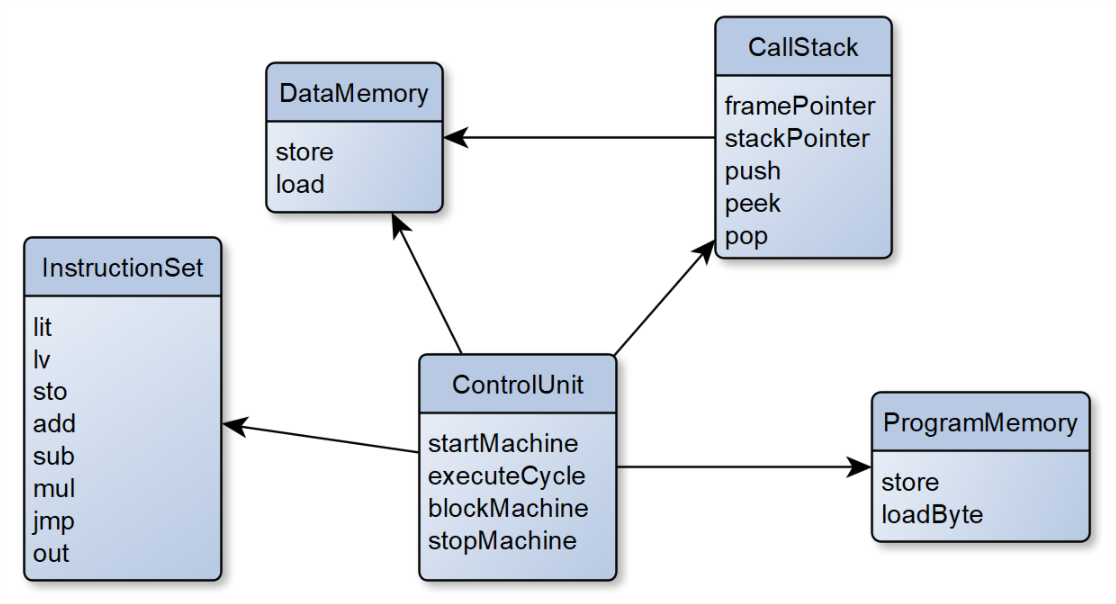
\includegraphics[scale=.62]{images/componentsOfNbM.png}
	\caption{Components of the NoBeardMachine Architecture}
	\label{fig:componentsOfNbM}
\end{figure}
\subsection{Program Memory}
The program memory stores instructions with \bau{their corresponding opcodes and operands.} belonging opcode and operands. \bau{The memory is byte addressed with a specified \ldots} It is byte addressed memory with a specified maximum size. Addresses access outside the range of 0 to the maximum size -1 lead to a “ProgramAddressError”. \bau{this is not really readable: Memory access outside the valid range lead to a \ldots? Furthermore: be consistent how parts of source code is formatted. I would strongly suggest to use the lstlisting environments.}

\subsection{Data Memory} \label{ssec:dataMemory} \bau{I would suggest to prefix labels only with sec:dataMemory. If you do your name spaces in such a granular way you loose too much of flexibility}
The data memory is a byte addressed storage and stores variables as follows:

\begin{itemize}
\item \textbf{Characters} are one-byte values \bau{and consume exactly one byte in memory, i.e., no alignment is done.}are stored byte wise into the data memory. 
\item \textbf{Integers }are four-byte values and stored in little endian order. Negative integer values are stored as Two’s Complement (see \cite{wikipedia_twos_2018}).
\item \textbf{Booleans }are four-bytes values and are stored as the integer 0 for false and the integer 1 for true.
\end{itemize}

\begin{figure}
\begin{center}
\begin{tabular}{p{8em}|p{8em}|}
\cline{2-2}
\parbox[t][3em][t]{8em}{\hfill 0} & String Constants \\[3em] \cline{2-2}
& Stack frame 1 \\[2em] \cline{2-2}
& Stack frame 2 \\[2em] \cline{2-2}
& \ldots \\[2em] \cline{2-2}
\parbox[b][4em][b]{8em}{\hfill MAX\_DATA} & free \\ \cline{2-2}
\end{tabular}
\end{center}
\caption{Data Memory of the NoBeard Machine}\label{fig:datamemory}
\end{figure}

As figure~\ref{fig:datamemory} shows, the data memory is separated into two parts, string constants and to stack frames of the currently running functions. 

\subsubsection{String Constants}
\bau{Hmh, this I do not understand: We are talking about the memory but suddenly you switch to the structure of NoBeard assembler programs}
String constants in NoBeard assembler programs  are \bau{stored} written at the beginning of the source code under quotation marks. It includes all strings that has to be printed out on the console. Before starting a program on the virtual machine string constants are stored in the constant memory. 

\subsubsection{Stack Frames}
After the constant memory the stack frames are maintained in a certain way \bau{why in a certain way?}. For every execution of a function a new frame is added \bau{Whenever a function gets called \ldots}. It holds data for the function arguments, local variables and its expression stack. As soon as \bau{a} function ends, its frame is removed. 

\begin{figure}
\begin{center}
\begin{tabular}{p{8em}|p{4em}|p{15em}}
\parbox[b][1em][b]{8em}{\hfill \cellcolor{Gray}\textcolor{White}{Address}} & \cellcolor{Gray}\textcolor{White}{Content} & \cellcolor{Gray}\textcolor{White}{Remark} \\ \cline{2-2} 
\cline{2-2}
\parbox[t][1em][t]{5em}{\hfill 0} & 0 & frame pointer of frame 0 \\ \cline{2-2}
& \ldots \\ \cline{2-2}
\parbox[t][1em][t]{5em}{\hfill 32} & 13 & local int in frame 0 \\ \cline{2-2}
\parbox[t][1em][t]{5em}{\hfill 36} & 0 & static link to frame 0 (start of frame 1)\\ \cline{2-2}
& \ldots \\ \cline{2-2}
\parbox[t][1em][t]{5em}{\hfill 68} & 17 & local int in frame 1\\ \cline{2-2}
\parbox[t][1em][t]{5em}{\hfill 72} & 42 & local int in frame 1\\ \cline{2-2}
\parbox[t][1em][t]{5em}{\hfill 76} & 36 & static link to frame 1 (start of frame 2) \\ \cline{2-2}
& \ldots \\ \cline{2-2}
\parbox[t][1em][t]{5em}{\hfill 108} & `D' \\ \cline{2-2}
\parbox[t][1em][t]{5em}{\hfill 109} & 61 \\ \cline{2-2}
\parbox[b][4em][b]{8em}{\hfill MAX\_DATA} & free \\ \cline{2-2}
\end{tabular}
\end{center}
\caption{Snapshot of a call stack with three frames}\label{fig:threeframes}
\end{figure}

\bau{Well this example does mainly explain how the assembler instruction la works. At this point of the thesis it appears a bit unmotivated.}
Figure~\ref{fig:threeframes} shows a pretty good example from \cite{bauer_p._2017}. Here we can see that the memory is working with three frames. Frame~0 starts at address 0. The first 32 bytes of each frame are reserved for administrative data like the static link and the dynamic link to the surrounding frame, the return value, etc. Address~32 holds the value of a local variable in frame~0.

\lstset{language=NoBeardAsm}

At address~36 frame~1 starts with the address to its statically surrounding frame, i.e, the function (or unit or block) represented by frame~0 is defining the function (or block) represented by frame~1. Frame~1 defines two local values at addresses 68 and 72. Now it can be easily verified that an assembler instruction \lstinline$la 0 32$ (see section~\ref{sec:instructions}) loads the value of the local (i.e., relative to the closest frame pointer) address 32. In the concrete example this is address $36 + 32 = 68$.

\subsection{Call Stack}
By structuring the data memory as a stack the call stack is needed as an abstraction to the data memory. With the help of different functions the call stack is able to add and remove frames from the stack and to maintain the expression stack. Data that are needed for each statement get stored in the expression stack. It grows and shrinks as needed and is empty at the end of each statement\bau{which statement do you mean here? Assembler statement, NoBeard Statement?}. The stack is addressed word-wise only. The call stack has the two major components:

\begin{itemize}
\item \textbf{Stack Pointer: }Address of the start of the last used word on the stack. 
\item \textbf{Frame Pointer: }Address of the first byte of the currently running function's stack frame. 
\end{itemize}

\subsection{Control Unit}
It is responsible for the program work flow. It executes one machine cycle in three steps, it fetches, decodes and operates the current instruction. Depending on some instruction, the control unit also affect the state of the machine. To achieve these steps it has to work with the following components:

\begin{itemize}
\item \textbf{Program Counter: }Start address of the next instruction to be executed.
\item \textbf{Machine State: }The NoBeard machine has four different states and is always in one of them. 
	\begin{itemize}
		\item \lstinline$running$: The machine runs
		\item \lstinline$stopped$: The machine stops. Usually when the end of program is reached.
		\item \lstinline$blocked$: The machine pauses. Mostly when a breakpoint is placed by the user.
		\item \lstinline$error$: Error state
	\end{itemize}
\end{itemize}

\section{Binary File Format}
The virtual machine runs only NoBeard object files with extension \lstinline$.no$ which can be generated by an NoBeard Assembler or NoBeard Compiler. From the first byte onwards the machine instructions are stored in a continuous flow. After a final \lstinline$halt$ instruction the stream of string constants is stored. This is also shown in figure~\ref{fig:binaryfileformat}.

\begin{figure}[h]
\begin{center}
\begin{tabular}{p{8em}|p{8em}|}
\cline{2-2}
\parbox[t][3em][t]{8em}{\hfill 0} & Instructions \\[3em] \cline{2-2}
\parbox[b][2em][b]{8em}{\hfill N} & String Constants \\ \cline{2-2}
\end{tabular}
\end{center}
\caption{NoBeard Binary File Format}\label{fig:binaryfileformat}
\end{figure}

\section{Runtime Structure of NoBeard Program}
\bau{This section is closely related to the section dealing with the control unit. Maybe it is better to merge these two}
The machine has a firmly defined execution cycle:
\begin{enumerate}
\item Fetch instruction
\item Decode instruction
\item Execute instruction
\end{enumerate}
The very first instruction is fetched from a specified starting program counter which is provided as an argument when starting the program. From this point of time forwards the program is running until the machine state changes from run. There are two options to interrupt the machine from running state. It get interrupted mostly by the debugger with a breakpoint. Or otherwise when the \lstinline$halt$ instruction get executed.
\section{Instructions}\label{sec:instructions}
\bau{As you informed me: This and the next section look like being not really finished yet.}
NoBeard instructions have a variable length and each one has an opcode and operands with an amount of between 0 and 2. For all instructions the first byte is dedicated to the op code, which is the id by which the instruction is identified on machine language level. The remaining bytes, if any, are dedicated to the operands of the instruction. 
\section{NoBeard Assembler}
To write programs for the NoBeard machine an Assembler is provided. NoBeard Assembler files are separated in two blocks, which is called the string constants and the assembler program. The files have the extensions .na for NoBeard Assembler. The string constants are stored between two double quotes and has to be located at the beginning of the file. There is no possibility to address one single constant, so when using a string constant in the assembler program one has to provide the start address of the string constant and the length needed in the program.  Assembler programs contains a sequence of assembler instructions. The programmer has to follow the instruction format as shown in the figure